\lstset{
	basicstyle=\fontsize{8}{10}\linespread{0.8}\lstfont,
	language=sql, % Или другой ваш язык -- см. документацию пакета
	commentstyle=\color{comment},
	numbers=left,
	numberstyle=\tiny,
	stepnumber=1,
	numbersep=5pt,
	xleftmargin =.19in,
	tabsize=4,
	extendedchars=\true,
	breaklines=true,
	keywordstyle=\color{black},
	frame=single,
	stringstyle=\lstfont\color{black}\lstfont,
	showspaces=false,
	showtabs=false,
	showstringspaces=false,
	showstringspaces=false,
	inputencoding=utf8x,
	keepspaces=true,
	captionpos=t,
	breakatwhitespace=false,
}

\section{Технологическая часть}
\subsection{Выбор языка программирования}
В качестве языка программирования был выбран С\#, так как:
\begin{enumerate}
    \item данный язык программирования объектно-ориентирован;
    \item имеется навыки использования данного языка программирования.
\end{enumerate}

\hfill

В качестве среды разработки была выбрана «Visual Studio 2022», так как:
\begin{enumerate}
    \item студенты могут использовать бесплатно;
    \item она имеет множество удобств, которые облегчают процесс написания и отладки кода;
    \item она обеспечивает работу с Windows Forms --- интерфейсом, который упрощает доступ к элементам интерфейса Microsoft Windows за счет создания обертки для существующего Win32 API в управляемом коде;
    \item я знаком с данной средой разработки, что сократит время изучения возможностей среды.
\end{enumerate}
\subsection{Сведения о модулях программы}
Программа состоит из следующих модулей:
\begin{itemize}[label = ---]
    \item Program.cs --- главная входная точка в программу; 
    \item Form.cs --- интерфейс программы;
    \item trafficlight.cs --- описывает систему светофоров для машин, метод преобразования цвета светофора для машин;
    \item pedestrialight.cs --- описывает систему светофоров для пешеходов, метод преобразования цвета светофора для пешеходов;
    \item car.cs --- описывает информации о машинах.
\end{itemize}

\subsection{Реализация программы}
Ниже, на листинге \ref{lst:tl} - \ref{lst:car}, приведены реализации классов, сделанны студентом Динь Вьет Ань.
\begin{lstlisting}[caption = Класс trafficlight, label = {lst:tl}]
class trafficlight
{
    public PictureBox y;
    public int yellowtime = 2;
    public int total;
    public PictureBox r;
    public PictureBox g;
    public int redtime = 8;
    public int greentime = 5;
    public int counter = 0;
    public trafficlight(PictureBox red1, PictureBox green1, PictureBox yellow1, Queue queue)
    {
        r = red1;
        g= green1;
        y = yellow1;
        total = yellowtime + greentime;
        y.Visible = false;
    }
    public virtual void turnongreen()
    {
        r.Visible = false;
        g.Visible = true;
        y.Visible = false;
    }
    public virtual void turnonred()
    {
        r.Visible = true;
        g.Visible = false;
        y.Visible = false;
    }
    public void turnonyellow()
    {
        r.Visible = false;
        g.Visible = false;
        y.Visible = true;
    }
    public void switchcolor1(pedestrialight ps1, pedestrialight ps2)
    {
        if (r.Visible == true && redtime <= counter && ps1.r.Visible == true && ps2.r.Visible == true)
        {
            turnongreen();
            counter = 0;
        }
        else
        {
            if (g.Visible == true && counter >= greentime)
            {
                turnonyellow();                   
                counter = 0;
            }
            else
                if (y.Visible == true && counter >= yellowtime)
                {
                    turnonred();                     
                    counter = 0;
                }
        }
    }
}
\end{lstlisting}

\begin{lstlisting}[caption = Класс pedestrialight, label = {lst:pl}]
class pedestrialight
{
    public trafficlight tl;
    public PictureBox r;
    public PictureBox g;
    public int redtime = 8;
    public int greentime = 5;
    public int counter = 0;
    public virtual void turnongreen()
    {
        r.Visible = false;
        g.Visible = true;
    }
    public virtual void turnonred()
    {
        r.Visible = true;
        g.Visible = false;
    }
    public pedestrialight(PictureBox red, PictureBox green, trafficlight traffic)        
    {
        r = red;
        g = green;
        tl = traffic;
        redtime = traffic.greentime + traffic.yellowtime;
        greentime = traffic.redtime;
    }
    public virtual void switchcolor(trafficlight tl1, trafficlight tl2, trafficlight tl3)
    {
        if (r.Visible == true && redtime <= counter && (tl1.r.Visible == true || tl1.y.Visible == true) && (tl2.r.Visible == true || tl2.y.Visible == true) && (tl3.r.Visible == true || tl3.y.Visible == true))
        {
            turnongreen();
            counter = 0;
        }
        else
            if (g.Visible == true && greentime == counter)
            {
                turnonred();
                counter = 0;
            }
    }
}  
\end{lstlisting}

\begin{lstlisting}[caption = Класс car, label = {lst:car}]
class car
{
    public PictureBox pb =  new PictureBox();
    public int direction, road, road1Ylim = 200, mid = 250, XFINAL=0, YFINAL=0;
    bool cross = false;
    int[] lst;
    int index;
    public car(int X0, int Y0, int r, int dir)
    {
        pb.SizeMode = PictureBoxSizeMode.StretchImage;
        pb.BackColor = Color.Transparent;
        pb.BackgroundImage = Properties.Resources.b;
        pb.Anchor = AnchorStyles.Left;
        pb.Location = new Point(X0, Y0);
        pb.Visible = true;
        direction = dir;
        road = r;
    }
    public bool passed ()
    {
        if (road == 1)
            if (pb.Location.Y >= road1Ylim) return true;
            else return false;
        else
            if (road == 2)
                if (pb.Location.X <= road1Ylim) return true;
                else return false;
        if (road == 3)
            if (pb.Location.X >= road1Ylim) return true;
            else return false;
        if (road == 4)
            if (pb.Location.Y <= road1Ylim) return true;
            else return false;
        return false;
    }
    public bool middle()
    {
        if (road == 1)
            if(pb.Location.Y >= mid) return true;
            else return false;
        if (road == 2)
           if (pb.Location.X<= mid) return true;
           else return false;
        if (road == 3)
            if (pb.Location.X >= mid) return true;
            else return false;
        if (road == 4)
            if (pb.Location.Y <= mid) return true;
            else return false;                           
        return false;
    }
    public bool crash()
    {
        if (road == 1 && !passed()&&index > 0)
            if ((pb.Location.Y + pb.Size.Height + 20) > lst[index-1])
                return true;
        if (road == 2 && !passed() && index > 0)
            if ((pb.Location.X - 20-pb.Size.Width ) < lst[index - 1])
                return true;
        if (road == 3 && !passed() && index > 0)
            if ((pb.Location.X + pb.Size.Width + 20) > lst[index - 1])
                return true;
        if (road == 4 && !passed() && index > 0)
            if ((pb.Location.Y -pb.Size .Height -20) < lst[index - 1])
                return true;
        return false;
    }
    public int move(trafficlight traffic, int[] l,int i)
    {
        lst = l;
        index = i;
        if(road == 1)
        {  
            if( !crash())
                if (!passed() || (cross && !middle()))
                    pb.Top += 10;
                else
                    if (traffic.g.Visible) cross = true;
            if (middle())
            {
                if (direction == 1) pb.Left -= 20; 
                if (direction == 2) pb.Left += 20;
                if (direction == 3) pb.Top += 20;
                return 10000;
            }
            return pb.Location.Y;                    
        }
        if (road == 2)
        {
            if (!crash())
                if (!passed() || (cross && !middle()))
                    pb.Left -= 10;
                else if (traffic.g.Visible) cross = true;
            if (middle())
            {
                if (direction == 1) // go left
                    pb.Top += 20;
                if (direction == 2)// go right
                    pb.Top -= 20;
                if (direction == 3)// go straight
                    pb.Left -= 20;
                return 0;
            }
            return pb.Location.X;
        }
        if (road == 3)
        {
            if (!crash())
                if (!passed() || (cross && !middle()))
                    pb.Left += 10;
                else
                    if (traffic.g.Visible) cross = true;
            if (middle())
            {
                if (direction == 1) // go left
                    pb.Top -= 20;
                if (direction == 2)// go right
                    pb.Top += 20;
                if (direction == 3)// go straight
                    pb.Left += 20;
                return 10000;
            }
            return pb.Location.X;
        }
        if (road == 4)
        {
            if (!crash())
                if (!passed() || (cross && !middle()))
                    pb.Top -= 10;
                else
                    if (traffic.g.Visible) cross = true;
            if (middle())
            {
                if (direction == 1) // go left
                    pb.Left -= 20;
                if (direction == 2)// go right
                    pb.Left += 20;
                if (direction == 3)// go straight
                    pb.Top-= 20;
                return 0;
            }
            return pb.Location.Y;
        }
        return pb.Location.X;
    }
}
\end{lstlisting}

\subsection{Примеры работы программы}
Ниже, на таблице \ref{img:s14} - \ref{img:s15}, приведены интерфейсы работы программы, сделанны студентом Ву Минь Куанг.
\begin{figure}[H]
	\begin{center}
		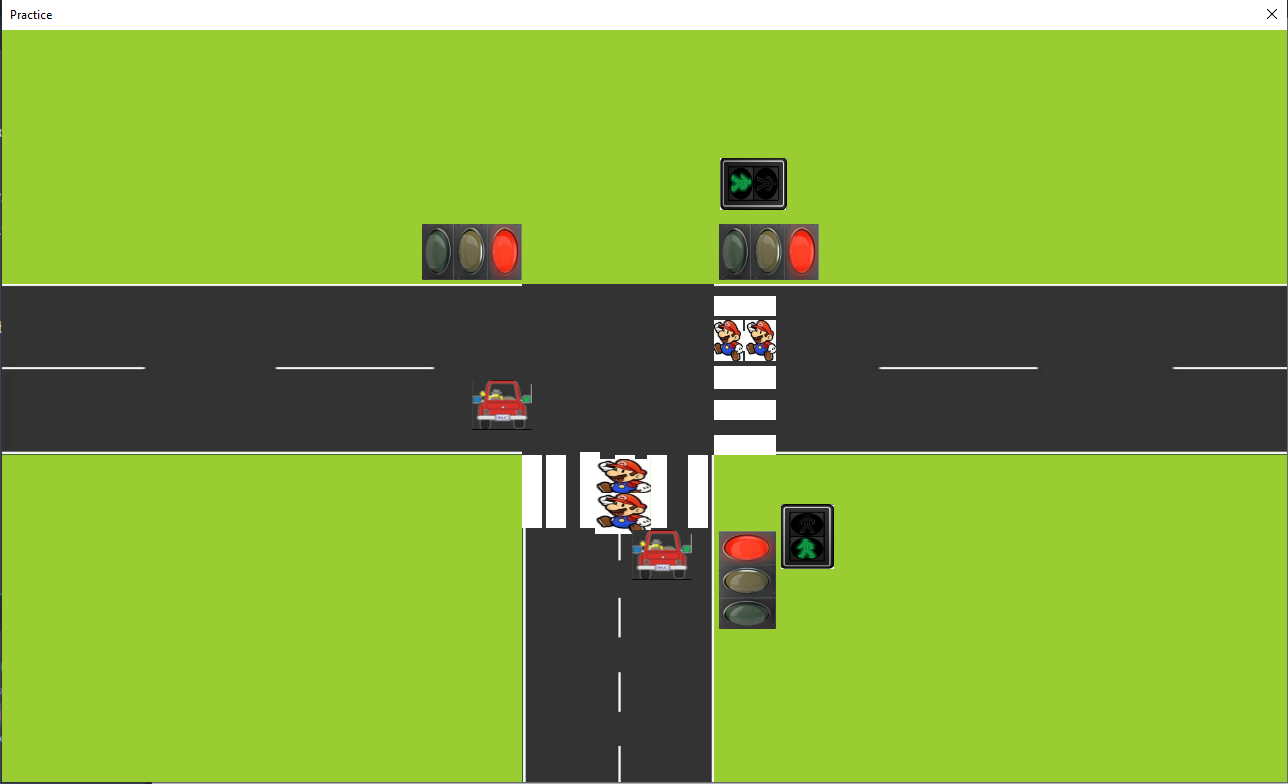
\includegraphics[scale=0.45]{img/prac1.png}
	\end{center}
	\captionsetup{justification=centering}
	\caption{Интерфейс работы программы.}
	\label{img:s14}
\end{figure}

\begin{figure}[H]
	\begin{center}
		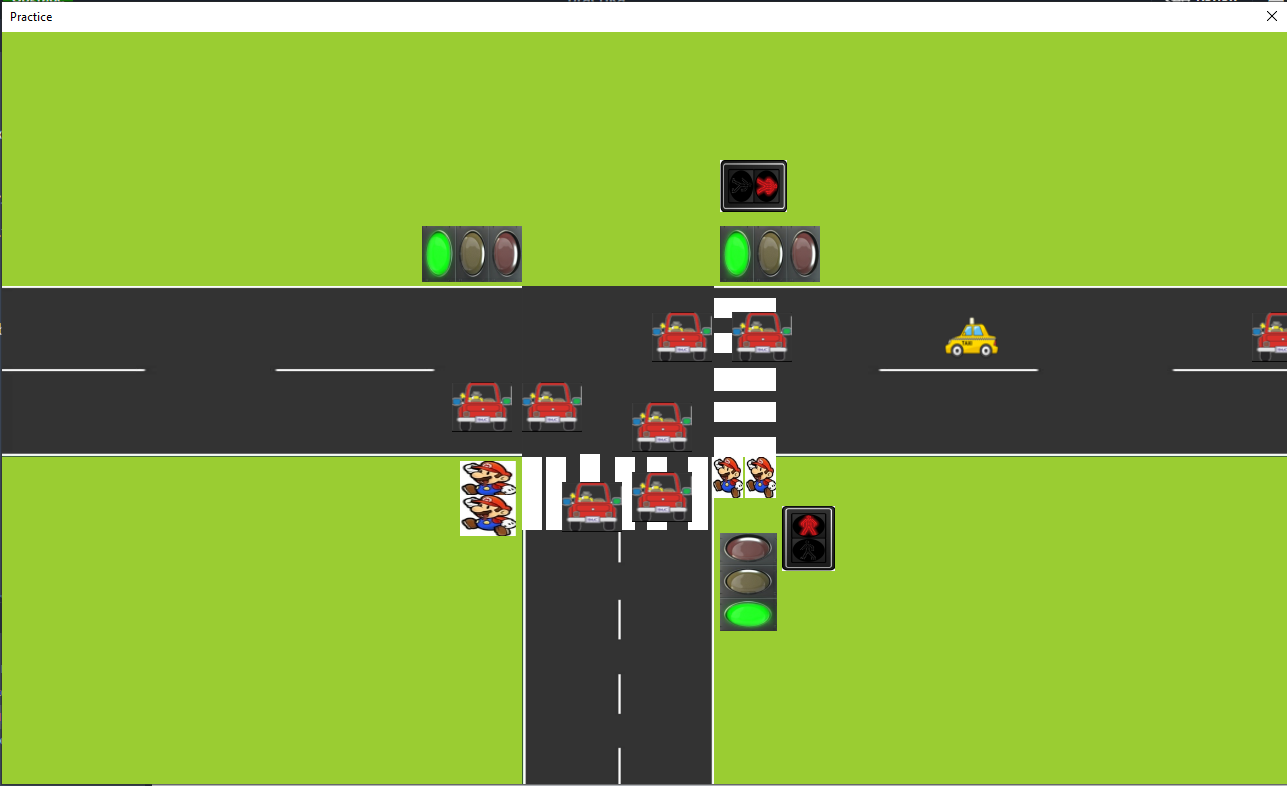
\includegraphics[scale=0.45]{img/prac2.png}
	\end{center}
	\captionsetup{justification=centering}
	\caption{Интерфейс работы программы.}
	\label{img:s15}
\end{figure}